%%%%%%%%%%%%%%%%%%%%%%%%%%%%%%%%%%%%%%%%%%%%%%%%%%%%%%%%%%
%%
%%  LOD-L5.tex
%%  Lecture 5: Cartan-De-Rham Calculus
%%
%%%%%%%%%%%%%%%%%%%%%%%%%%%%%%%%%%%%%%%%%%%%%%%%%%%%%%%%%%

\chapter*{\S L5. Cartan-De-Rham Calculus}
\setcounter{footnote}{0}

%%%%%%%%%%%%%%%%%%%%%%%%%%%%%%%%%%%%%%%%%%%%%%%%%%%%%%%%%%
%%
%% MARK: Abstract
%%
%%%%%%%%%%%%%%%%%%%%%%%%%%%%%%%%%%%%%%%%%%%%%%%%%%%%%%%%%%
\begin{abstract}
  This lecture is about the crucial theory of differential calculus,
  also called Cartan calculus.
  It is accompanied with the description of the De Rham Cohomology and its principal properties.
\end{abstract}

%%%%%%%%%%%%%%%%%%%%%%%%%%%%%%%%%%%%%%%%%%%%%%%%%%%%%%%%%%
%%
%% MARK: Introduction
%%
%%%%%%%%%%%%%%%%%%%%%%%%%%%%%%%%%%%%%%%%%%%%%%%%%%%%%%%%%%

In this lecture we shall see the elementary constructions and definitions of the theory of differential calculus in diffeology.
In particular,
a reminder about smooth forms in Euclidean spaces,
the definitions of differential forms in diffeology,
the operations of pullbacks and exterior differential,
the behavior under subduction with an example on orbifold,
the definition of the De Rham cohomology,
the definition of the cubic homology and the integration of forms on chains,
the De Rham homomorphism.

%%%%%%%%%%%%%%%%%%%%%%%%%%%%%%%%%%%%%%%%%%%%%%%%%%%%%%%%%%
%%
%% MARK:  Smooth Forms in Euclidean Spaces
%%
%%%%%%%%%%%%%%%%%%%%%%%%%%%%%%%%%%%%%%%%%%%%%%%%%%%%%%%%%%
\section{Smooth forms in Euclidean spaces}

\begin{Article}{Linear $p$-forms on $\RR^n$.}{}
  A \emph{linear $p$-form} on the Euclidean space $\RR^n$ is a map
  $$%
    \alpha \colon (\RR^n)^p \to \RR
  $$%
  which is \emph{multilinear},
  that is,
  linear in each parameter,
  \begin{eqnarray*}
    \alpha(v_1,\dots, \lambda v_i + \mu v'_i,\dots,v_p)  & = & \lambda \alpha(v_1,\dots,v_i,\dots,v_p)\\
    & + & \mu \alpha(v_1,\dots,v'_i,\dots,v_p)
  \end{eqnarray*}
  for all $i=1\dots p$,
  and which is antisymmetric under every \emph{transposition},
  $$%
    \alpha(v_1,\dots,v_i, \dots,v_j,\dots,v_p) = - \alpha(v_1,\dots,v_j, \dots,v_i,\dots,v_p).
  $$%
  We deduce from the antisymmetry that for all \emph{permutations} $\epsilon$ of $\{1,\dots,p\}$
  $$%
    \alpha(v_{\epsilon(1)},\dots,v_{\epsilon(p)}) = (-1)^{\Sign(\epsilon)} \alpha(v_1,\dots,v_p),
  $$%
  where $\Sign$ denotes the \emph{signature} of the permutations.

  We denote
  $$%
    \Lambda^p(\RR^n)
  $$%
  the set of $p$-forms (a shortcut for linear $p$-forms).
  This set is naturally a real vector space:
  $$%
    (\lambda \alpha + \mu \beta)(v_1,\dots,v_p) = \lambda \alpha(v_1,\dots,v_p) + \mu \beta(v_1,\dots,v_p).
  $$%
  Note that:
  $$%
    \Lambda^0(\RR^n) = \RR
    \SpacedText{and}
    \Lambda^1(\RR^n) = (\RR^n)^* \simeq \RR^n,
  $$%
  the \emph{dual space} of $\RR^n$.
  The dimension is the binomial coefficient
  $$%
    \dim(\Lambda^p(\RR^n))  = {n! \over p! \ (n-p)!}.
  $$%
  Note that:
  $$%
    \dim(\Lambda^n(\RR^n)) = 1
    \SpacedText{and}
    \dim(\Lambda^p(\RR^n)) = 0
    \SpacedText{if $p>n$.}
  $$%

  \uline{Note.} Sometimes I write
  $$%
    \alpha(v_1)\cdots(v_p)
    \SpacedText{for}
    \alpha(v_1,\cdots,v_p).
  $$%
\end{Article}

\begin{Article}{Pullbacks of linear forms.}{}
  Consider a linear map
  $$%
    M \colon \RR^n \to \RR^m
  $$%
  Let $\beta \in \Lambda^p(\RR^m)$,
  We call \emph{pullback} of $\beta$ by $M$ the map denoted and defined by
  $$%
    M^*(\beta) (v_1,\dots,v_p) = \beta(M v_1,\dots, M v_p).
  $$%
  The map $M^*(\beta)$ is obviously a linear $p$-form on $\RR^n$.
  Moreover,
  $M^*$ is linear:
  $$%
    M^*  \in \L\big(\Lambda^p(\RR^m),\Lambda^p(\RR^n)\big).
  $$%
\end{Article}

\begin{Article}{Smooth forms on Euclidean domains.}{}
  Let $U \subset \RR^n$,
  we call \emph{smooth $p$-form} on $U$ any smooth map
  $$%
    \alpha \colon U \to \Lambda^p(\RR^n).
  $$%
  We denote by a bold letter $\SmoothForms$ the space of smooth forms on $U$,
  $$%
    \SmoothForms^p(U) = \Cinfty\big(U,\Lambda^p(\RR^n)\big).
  $$%
  In this case:
  $\alpha \in \SmoothForms^p(U)$,
  $\alpha(x) \in \Lambda^p(\RR^n)$ for all $x \in U$.

  There are a few ways of defining ``smooth'' for a $p$-form,
  one can use the canonical decomposition of a linear $p$-form on the canonical basis
  (it is documented everywhere,
  and also in \cite{PIZ13}),
  or we can directly define it by this property:
  $$%
    \text{For all } v_1,\dots,v_p \in \RR^n
    \quad
    [x \mapsto \alpha(x)(v_1,\dots,v_p)] \in \Cinfty(U, \RR).
  $$%
  The expression $\alpha(x)(v_1,\dots,v_p)$ reads:
  $\alpha$ at the point $x$ applied to the vectors $v_1,\dots,v_p$.

  \uline{Note 1.} For $p=0$ we have simply
  $$%
    \SmoothForms^0(U) = \Cinfty(U,\RR).
  $$%

  \uline{Note 2.} The set $\SmoothForms^p(U)$ is obviously a vector space.
  It can be equipped with a functional diffeology that extends the functional diffeology on $\SmoothForms^0(U) = \Cinfty(U,\RR)$.
\end{Article}

\begin{Article}{Pullback of a smooth form.}{}
  Let $U \in \RR^n$ and $U' \in \RR^{n'}$,
  let $f \in \Cinfty(U,U')$ and $\beta \in \SmoothForms^p(U')$.
  We call \emph{pullback} of $\beta$ by $f$,
  and we denote by $f^*(\beta)$ the $p$-form on $U$ defined by:
  $$%
    f^*(\beta)(x)(v_1,\dots,v_p) = \beta(f(x))(M v_1,\dots,M v_p),
    \text{ with }
    M = \Der(f)(x),
  $$%
  for all $x \in U$ and all $v_1,\dots, v_p\in \RR^n$.

  Then,
  $f^*(\beta)$ is a smooth $p$-form on $U$,
  $$%
    \forall \beta \in \SmoothForms^p(U'),
    \quad
    f^*(\beta) \in \SmoothForms^p(U).
  $$%
  Moreover $f^*$ is a linear operator:
  $$%
    f^*(\lambda \alpha + \mu \beta) = \lambda f^*(\alpha) + \mu f^*(\beta),
  $$%
  and smooth for the functional diffeology.
\end{Article}

\begin{Article}{Exterior derivative of a smooth form.}{}
  \label{Exterior-derivative-of-a-smooth-form}
  Let $\alpha$ be a $p$-form,
  $$%
    \alpha \in \SmoothForms^p(U),
  $$%
  on a domain $U \subset \RR^n$.

  Let $d\alpha$ be defined as follows:
  \allowdisplaybreaks
  \begin{eqnarray*}
    d\alpha(x)(v_0,v_1,\dots,v_p) & = & {\partial \alpha(x)(v_1,v_2,v_3,\dots,v_p) \over \partial x}(v_0) \\
    & - & {\partial \alpha(x)(v_0,v_2,v_3,\dots,v_p) \over \partial x}(v_1) \\
    & - & {\partial \alpha(x)(v_1,v_0,v_3\dots,v_p) \over \partial x}(v_2) \\
    & - & {\partial \alpha(x)(v_1,v_2,v_0,\dots,v_p) \over \partial x}(v_3) \\
    & - & \cdots \\[1ex]
    & - & {\partial \alpha(x)(v_1,v_2,\dots,v_{p-1},v_0) \over \partial x}(v_p).
  \end{eqnarray*}
  where $v_0,v_1,\dots,v_p \in \RR^n$.

  Then,
  $$%
    d\alpha \in \SmoothForms^{p+1}(U)
    \SpacedText{and}
    d[d\alpha] = 0,
  $$%
  for all $\alpha$.
  The $(p+1)$-form $d\alpha$ is called the \emph{exterior derivative},
  or \emph{exterior differential},
  of $\alpha$,
  and the operator
  $$%
    d \colon \SmoothForms^p(U) \to \SmoothForms^{p+1}(U)
  $$%
  is called the \emph{exterior differentiation}.

  \uline{Note 1.} for $f \in \DForms^0(U) = \Cinfty(U,\RR)$,
  $$%
    df(x) \colon v \mapsto {\partial f(x) \over \partial x}(v).
  $$%
  \uline{Note 2.} For $n = 2$ and $p=1$
  $$%
    \alpha = a(x,y) dx + b(x,y) dy,
  $$%
  where $dx(v) = v^x$ and $dy(v) = v^y$ are the coordinate $1$-forms,
  with $v= (v^x,v^y)$.
  We have:
  $$%
    d\alpha(x)(v_1,v_2) = \bigg({\partial b(x,y) \over \partial x} - {\partial a(x,y) \over \partial y} \bigg) (v_1^x v_2^y - v_2^x v_1^y).
  $$%
  The linear $2$-form
  $$%
    (v_1,v_2) \mapsto v_1^x v_2^y - v_2^x v_1^y
  $$%
  is denoted by $dx \wedge dy$,
  such that
  $$%
    d\alpha(x) = \bigg({\partial b(x,y) \over \partial x} - {\partial a(x,y) \over \partial y}\bigg) dx \wedge dy.
  $$%
  \uline{Note 3.} Pullback and exterior differentiation commute:
  $$%
    f^*(d\alpha) = d[f^*(\alpha)].
  $$%
\end{Article}

%%%%%%%%%%%%%%%%%%%%%%%%%%%%%%%%%%%%%%%%%%%%%%%%%%%%%%%%%%
%%
%% MARK:  Differential Forms in Diffeology
%%
%%%%%%%%%%%%%%%%%%%%%%%%%%%%%%%%%%%%%%%%%%%%%%%%%%%%%%%%%%
\section{Differential forms in diffeology}

\begin{Article}{Differential forms.}{}
  Let $X$ be a diffeological space.
  A differential $p$-form on $X$ is a mapping
  $$%
    \alpha \colon P \mapsto \alpha(P),
  $$%
  for all plots $P$ in $X$ such that:

  \begin{enumerate}
    \item $\alpha(P) \in \SmoothForms^p(U)$,
    with $U = \Domain(P)$.
    \item For all Euclidean domains $V$,
    for all $F \in \Cinfty(V,U)$,
    $$%
      \alpha(P \circ F) = F^*(\alpha(P)).
    $$%
  \end{enumerate}

  The set of differential $p$-forms on $X$ is a vector space denoted by
  $$%
    \DForms^p(X).
  $$%
  It can be equipped with a natural functional diffeology that extends the functional diffeology on
  $$%
    \DForms^0(X) = \Cinfty(X,\RR).
  $$%
  %
  \uline{Note.} When we consider the Euclidean domain $U$ as a diffeological space,
  then a differential form $\alpha$ is naturally identified with the value
  $$%
    \underline{\alpha} = \alpha(\Id_{U}).
  $$%
  We will then identify naturally $\SmoothForms^p(\U) \simeq \DForms^p(U)$.
\end{Article}

\begin{Article}{Pullback of a differential form.}{}
  Let $X$ and $X'$ be two diffeological spaces.
  let $\beta \in \DForms^p(X')$ and $f \in \Cinfty(X,X')$.
  Then,
  for all plots $P$ in $X$
  $$%
    [f^*(\beta)](P) = \beta(f \circ P)
  $$%
  defines the pullback of $\beta$ by $f$,
  $$%
    \forall \beta \in \DForms^p(X'), \quad f^*(\beta) \in \DForms^p(X).
  $$%
  The pullback is linear and smooth.

  \uline{Note.} We can identify
  $$%
    \alpha(P) = P^*(\alpha).
  $$%
  We should more properly write $\alpha(P) = \uline{P^*(\alpha)} = P^*(\alpha)(\Id_U)$,
  where $U = \Domain(P)$.
\end{Article}

\begin{Article}{Exterior differential of a differential form.}{}
  Let $X$ be a diffeological space and $\alpha \in \DForms^p(X)$.
  Then,
  $$%
    d\alpha \colon P \mapsto d[\alpha(P)]
  $$%
  is a differential $(p+1)$-form on $X$.
  The operator $d$ is linear and smooth,
  for the functional diffeology.
  It satisfies
  $$%
    d \circ d = 0.
  $$%
\end{Article}

%%%%%%%%%%%%%%%%%%%%%%%%%%%%%%%%%%%%%%%%%%%%%%%%%%%%%%%%%%
%%
%% MARK:  Pushing Forwards Differential Forms
%%
%%%%%%%%%%%%%%%%%%%%%%%%%%%%%%%%%%%%%%%%%%%%%%%%%%%%%%%%%%
\section{Pushing forwards differential forms}

\begin{Article}{Pushing forms onto quotients.}{}
  \label{Pushing-forms-onto-quotients}
  Let $X$ and $X'$ be two diffeological spaces.
  Let $\pi: X \to X'$ be a subduction and let $\alpha$ be a differential $k$-form on $X$.

  \uline{Theorem.} {\itshape The $k$-form $\alpha$ is the pullback of a $k$-form $\beta$ defined on $X'$,
  $\alpha = \pi^*(\beta)$,
  if and only if,
  for any two plots $P$ and $Q$ of $X$ such that $\pi \circ P = \pi \circ Q$,
  then $\alpha(P) = \alpha(Q)$.}

  We also say that $\beta$ is the \emph{pushforward} of $\alpha$ by $\pi$.
  The differential forms of $X$ satisfying this property may be called \emph{basic forms},
  with respect to $\pi$.

  \uline{Note 1.} For every integer $k$,
  the pullback $\pi^*: \DForms^k(X') \to \DForms^k(X)$ is always a smooth linear map.
  The previous proposition is a characterization of the image of $\pi^*$, when $\pi$ is a subduction.

  \uline{Note 2.} This property can be expressed with the help of a diagram and it is used for integrating closed $2$-forms.
  Consider the pullback of $\pi$ by itself
  $$%
    \pi^*(X) = \{ (x_1,x_2) \in X \times X \mid \pi(x_1) = \pi(x_2)\},
  $$%
  with projections $\Proj_1$ and $\Proj_2$.
  \begin{center}
    \begin{tikzpicture}[ auto]
      \node (A)  at (0,0) {$\pi^*(X)$};
      \node (B)  at (3,0) {$X$};
      \node (C)  at (0,-2) {$X$};
      \node (D)  at (3,-2) {$X'$};
      \draw[->] (A) to node {$\Proj_1$} (B);
      \draw[->] (A) to node [swap] {$\Proj_2$} (C);
      \draw[->] (B) to node {$\pi$} (D);
      \draw[->] (C) to node [swap] {$\pi$} (D);
    \end{tikzpicture}
  \end{center}
  Then,
  $\alpha$ is basic with respect to $\pi$ if and only if $\Proj_1^*(\alpha) - \Proj_2^*(\alpha) = 0$,
  in other words,
  if and only if $\Proj_1^*(\alpha) = \Proj_2^*(\alpha)$.
\end{Article}

\begin{Article}{Vanishing forms on quotients.}{}
  Let $X$ and $X'$ be two diffeological spaces and $f \colon X \to X'$ be a subduction.
  Let $\alpha$ be a $p$-form on $X'$,
  $\alpha \in \DForms^p(X')$,
  $p \in \NN$.
  Then,
  $f^*(\alpha) = 0$ if and only if $\alpha = 0$.
  Equivalently,
  for any two $p$-forms $\alpha$ and $\beta$ on $X'$ and for every subduction $f$ from $X$ to $X'$,
  \begin{equation}
    \renewcommand{\theequation}{$\diamondsuit$}
    f^*(\alpha) = f^*(\beta) \quad \Rightarrow \quad \alpha = \beta.
  \end{equation}
  In other words,
  for every subduction $f \colon X \to X'$,
  the pullback by $f^* \colon \DForms^p(X') \to \DForms^p(X)$ is injective.

  \uline{Note.} This implies in particular that if a diffeological space $X$ has a finite dimension $n \in \NN$,
  then every $n+k$ differential form,
  with $k > 0$,
  is zero.
  Formally,
  \begin{equation}
    \renewcommand{\theequation}{$\heartsuit$}
    \dim(X) = n < \infty
    \SpacedText{implies}
    \DForms^{n+k}(X) = \{0\},
    \text{ for all $k>0$.}
  \end{equation}
\end{Article}

\begin{Article}{The corner orbifold.}{}
  Consider the \emph{corner orbifold}
  $$%
    \cQ = \Delta_1^2 = [\RR/\{\pm 1\}]^2 = \RR^2/ \{\pm 1\}^2.
  $$%
  Show that every $2$-form on $\cQ$ is proportional to the $2$-form $\omega$ defined on $\cQ$ by
  $$%
    \pi^*(\omega) = 4xy \, dx \wedge dy.
  $$%
  That is,
  for any other differential form $\omega' \in \DForms^2(\cQ)$,
  there exists a smooth function $\pphi \in \Cinfty(\cQ,\RR)$ such that $\omega' = f \omega$.
\end{Article}

\begin{proof}
  Let $\omega'$ be a $2$-form on $\cQ$,
  and let $\tilde \omega'$ be its pullback by $\pi$,
  $$%
    \tilde \omega' = \pi^*(\omega').
  $$%
  Thus,
  there exists a smooth real function $F$ such that
  $$%
    \tilde \omega' = F \times dx \wedge dy,
  $$%
  where $dx \wedge dy$ is the canonical basis on $\DForms^2(\RR^2)$.
  But since $\pi \circ (\epsilon,\epsilon') = \pi$,
  for all $(\epsilon,\epsilon') \in \{\pm 1\}^2$,
  we get
  $$%
    \epsilon \epsilon' F(\epsilon x,\epsilon' y) = F(x,y),
  $$%
  for all $(x,y) \in \RR^2$ and all $\epsilon$,
  $\epsilon'$ in $\{\pm1\}$.
  Thus,
  $F(-x,y) = -F(x,y)$ and $F(x,-y) = -F(x,y)$.
  In particular,
  $F(0,y) = 0$ and $F(x,0) = 0$.
  Therefore,
  since $F$ is smooth,
  there exists $f \in \Cinfty(\RR^2,\RR)$ such that $F(x,y) = 4xyf(x,y)$,
  with $f(\epsilon x, \epsilon' y) = f(x,y)$.
  Therefore,
  $\tilde \omega' = f \times \tilde \omega$,
  with
  $$%
    \tilde \omega = 4xy \times dx \wedge dy,
  $$%
  that is,
  $$%
    \tilde\omega = d(x^2) \wedge d(y^2),
  $$%
  but $x\mapsto x^2$ and $y \mapsto y^2$ are invariant by $\{\pm1\}^2$,
  so they are the pullback by $\pi$ of some smooth real functions on $\cQ$.
  Thus,
  $d(x^2)$ and $d(y^2)$ are the pullback of $1$-forms on $\cQ$,
  let us say
  $$%
    d(x^2) = \pi^*(ds)
    \SpacedText{and}
    d(y^2) = \pi^*(dt),
  $$%
  so,
  $\tilde \omega = \pi^*(\omega)$,
  where $\omega = ds \wedge dt$ is a well defined $2$-form on $\cQ$.
  Now,
  since $f(\epsilon x, \epsilon'y) = f(x,y)$ means just that $f$ is the pullback of a smooth real function $\pphi$ on $\cQ$,
  it follows that any $2$-form $\omega'$ on $\cQ$ is proportional to $\omega$,
  that is,
  $\omega' = \pphi \times \omega$,
  with $\pphi \in \Cinfty(\cQ,\RR)$.
\end{proof}

%%%%%%%%%%%%%%%%%%%%%%%%%%%%%%%%%%%%%%%%%%%%%%%%%%%%%%%%%%
%%
%% MARK:  De Rham Cohomology
%%
%%%%%%%%%%%%%%%%%%%%%%%%%%%%%%%%%%%%%%%%%%%%%%%%%%%%%%%%%%
\section{De Rham cohomology}

\begin{Article}{The De Rham cohomology.}{}
  \label{The-De-Rham-cohomology}
  Let $X$ be a diffeological space.
  The exterior derivative defined above satisfies the \emph{coboundary condition}
  $$%
    d: \DForms^p(X) \to \DForms^{p+1}(X),
    \ p \geq 0
    \SpacedText{and}
    d \circ d = 0.
  $$%
  As is usual in cohomology theories \cite{McL75},
  when we have a chain complex
  ---~here the chain complex of real vector spaces $\DForms^\star(X) = \{\DForms^p(X)\}_{p=0}^\infty$ with a coboundary operator $d$~---
  the space of \emph{$p$-cocycles} is defined as the kernel in $\DForms^p(X)$ of the operator $d$,
  and the space of \emph{$p$-coboundaries} is defined as the image,
  in $\DForms^p(X)$,
  of the operator $d$.
  They will be denoted by
   \vspace{.5ex}
   $$%
    \left\{
    \begin{array}{rcl}
    \ZDR^p(X) & = &\ker \left[d: \DForms^p(X) \to \DForms^{p+1}(X)\right], \\[1.5ex]
    \BDR^p(X) & = & d (\DForms^{p-1}(X))\subset \ZDR^p(X)
    \SpacedText{with}
    \BDR^0(X) = \{0\}.
    \end{array}
    \right.
  $$%
  The \emph{De Rham cohomology groups} of $X$ are then defined as the quotients of the spaces of cocycles by the spaces of coboundaries,
  we denote them by
  $$%
    \HDR^p(X) = \ZDR^p(X)/\BDR^p(X).
  $$%
  Since the operator $d$ is linear,
  and since the space of differential $p$-forms $\DForms^p(X)$,
  equipped with the functional diffeology,
  is a diffeological vector space,
  the De Rham cohomology group $\HDR^p(X)$,
  equipped with the quotient diffeology,
  is a diffeological vector space.
\end{Article}

\begin{Article}{Homotopy invariance of the De Rham cohomology.}{}
  Let $f : X \to X'$ be a smooth map.
  Since the exterior derivative commutes with the pullback,
  we have a morphism
  $$%
    f^\# : \HDR(X') \to \HDR(X)
  $$%
  with
  $$%
    f^\#(\Class(\alpha')) = \Class(f^*(\alpha')),
  $$%
  for all $\alpha' \in \DForms^*(X')$.
  We shall prove the following theorem in a later lecture.

  \uline{Theorem.} {\itshape If $s \mapsto f_s$ is an homotopy,
  that is,
  a smooth path in $\Cinfty(X,X')$,
  then
  $$%
    f_0^\# = f_1^\#.$$%
  }

  That is called the \emph{homotopy invariance} of the De Rham cohomology.

  \uline{Corollary} If $A$ is a \emph{deformation retract} of $X$,
  then the De Rham cohomology of $X$ coincides with the De Rham cohomology of $A$.
  Contractible spaces have a trivial cohomology.
\end{Article}

%%%%%%%%%%%%%%%%%%%%%%%%%%%%%%%%%%%%%%%%%%%%%%%%%%%%%%%%%%
%%
%% MARK:  Cubic Homology and De Rham Cohomology
%%
%%%%%%%%%%%%%%%%%%%%%%%%%%%%%%%%%%%%%%%%%%%%%%%%%%%%%%%%%%
\section{Cubic homology and De Rham cohomology}

\begin{Article}{Cubes and cubic chains in diffeological spaces.}{}
  \label{Cubes-and-cubic-chains-on-diffeological-spaces}
  A \emph{standard $p$-cube} is the subset $[0,1]^p$ of $\RR^p$,
  and we denote it by $\cub{p}$,
  $$%
    \cub{p} = [0,1]^p \subset \RR^p.
  $$%
  Let $X$ be a diffeological space.
  A \emph{smooth $p$-cube} in $X$ any smooth map from $\RR^p$ to $X$.
  And $\DCubes{p}(X)$ denotes the set of all the smooth $p$-cubes in $X$,
  $$%
    \DCubes{p}(X) = \Cinfty(\RR^p,X).
  $$%
  The set $\DCubes{p}(X)$ will be equipped with the functional diffeology.

  Note that since $0$-cubes are any maps from $\cub{0} = \RR^0 = \{0\}$ to $X$,
  then $\DCubes{0}(X)$ is naturally equivalent to $X$,
  thanks to the diffeomorphism $x \mapsto \bmx = [0 \mapsto x]$.
  Hence,
  $$%
    \DCubes{0}(X) \simeq X.
  $$%
  Then,
  we define the \emph{smooth cubic $p$-chains} in $X$,
  with coefficients in $\ZZ$,
  as the free Abelian group generated by $\DCubes{p}(X)$,
  and we denote it by $\DChains{p}(X)$.
  Thus,
  a (smooth) cubic $p$-chain $c$,
  in $X$,
  is any finite $\ZZ$-linear combination of $p$-cubes,
  that is,
  $$%
    c = \sum_\sigma n_\sigma \sigma,
    \text{ with } \sigma \in \DCubes{p}(X),
    \text{ and } n_\sigma \in \ZZ,
  $$%
  where the sum is performed over a finite set of $p$-cubes called the \emph{support} of $c$,
  and denoted by
  $$%
    \Supp(c) = \{ \sigma \in \DCubes{p}(X) \mid n_\sigma \neq 0 \}.
  $$%
  The group of cubic $p$-chains $\DChains{p}(X)$ can be represented by
  $$%
    \DChains{p}(X) \simeq \{ c \in  \Maps(\DCubes{p}(X),\ZZ) \mid \#\Supp(c) <\infty \}.
  $$%
  Note that in the writing $\sum_\sigma n_\sigma \sigma$ of the chain $c$,
  $n_\sigma = c(\sigma)$.
  Then,
  the sum of two cubic $p$-chains $c$ and $c'$,
  and the multiplication of a cubic $p$-chain $c$ by an integer $m$,
  are defined as usual:
  $$%
    (c + c')(\sigma) = c(\sigma)  + c'(\sigma)
    \SpacedText{and} (mc)(\sigma) = m \times c(\sigma).
  $$%
  \uline{Note 1.} A cubic chain can also be regarded as any finite family
  $$%
    \{(n_i,\sigma_i)\}_{i \in \cI}
  $$%
  and can be written $\sum_{i \in \cI} n_i \sigma_i$,
  with the convention that if $\sigma_i = \sigma_j$,
  then
  $$%
    \sum_{i \in \cI} n_i \sigma_i = \sum_{i' \in \cI'} n_{i'} \sigma_{i'} + (n_i + n_j)\sigma_i,
  $$%
  where $\cI' = \cI - \{i,j\}$.
  Since the family is finite,
  the sum of the coefficients of a same cube is finite and both aspects are equivalent.

  \uline{Note 2.} With smooth homology or cohomology in mind,
  there is no contradiction in defining smooth $p$-cubes in $X$ as smooth maps from $\RR^p$ to $X$,
  as we do here,
  or as the maps from $\cub{p}$ to $X$ which are the restrictions of smooth maps defined on an open neighborhood of $\cub{p}$,
  as we could have also chosen to do.
  Indeed the following proposition addresses this issue.

  \begin{enumerate}
    \item[($\diamondsuit$)] Every $p$-plot of $X$ defined on a small open neighborhood of $\cub{p}$ coincides,
    on $\cub{p}$,
    with some global $p$-plot of $X$.
  \end{enumerate}

  This is why,
  for sake of simplicity and without loss of generality,
  the smooth $p$-cubes in $X$ have been defined as the global $p$-plots of $X$.
  But to focus our attention on $\cub{p} \in \RR^p$ we have introduced a special name,
  $p$-cube instead of global $p$-plot,
  and a special notation $\DCubes{p}(X)$ for $\Cinfty(\RR^p,X)$.
\end{Article}

\begin{Article}{Boundary of cubes and chains.}{}
  Let us introduce the following family of injections,
  for all $a\in\RR$\,:
  $$%
    j_k(a) \colon \RR^p \to \RR^{p+1}, \ k = 1, \ldots, p+1,
  $$%
  defined by
  $$% \renewcommand{\arraystretch}{1.3}
    \begin{array}{crcl}
    k = 1 & j_1(a) \colon (t_1)\cdots(t_p) & \mapsto & (a)(t_1)\cdots(t_p), \\
    1 < k \leq p & j_k(a) \colon (t_1)\cdots(t_p) & \mapsto & (t_1)\cdots(t_{k-1})(a)(t_k)\cdots(t_p), \\
    k = p+1 & j_{p+1}(a): (t_1)\cdots(t_p) & \mapsto & (t_1)\cdots(t_p)(a).
    \end{array}
  $$%
  Given a $p$-tuple of numbers,
  $j_k(a)$ puts $a$ at the place number $k$,
  preserving the numbers before and shifting the numbers after.

  We define the boundary operator $\Boundary$,
  for $p \geq 1$,
  %
  \begin{equation}
    \renewcommand{\theequation}{$\diamondsuit$}
    \text{for all } \sigma \in \DCubes{p}(X),
    \quad \Boundary\sigma =  \sum_{k = 1}^p (-1)^k[\sigma \circ j_k(0) - \sigma \circ j_k(1)].
  \end{equation}
  %
  The operator $\Boundary$ defined by $(\diamondsuit)$ is naturally extended by linearity on all cubic $p$-chains,
  with $p \geq 1$.
  The boundary of the $p$-chain $c = \sum_\sigma n_\sigma \sigma$ is given by
  %
  \begin{equation}
    \renewcommand{\theequation}{$\heartsuit$}
    \Boundary c = \sum_\sigma n_\sigma \sum_{k = 1}^p (-1)^k[\sigma \circ j_k(0) - \sigma \circ j_k(1)].
  \end{equation}
  %
  The operator $\Boundary$ defined by $(\heartsuit)$ is a boundary operator,
  that is,
  $$%
    \Boundary \circ \Boundary = 0,$$%
  and we get the \emph{chain-complex}
  \begin{equation}
    \renewcommand{\theequation}{$\clubsuit$}
    \cdots
    {\buildrel\Boundary\over{\ \longrightarrow \ }}
    \DChains{p}(X)
    {\buildrel\Boundary\over{\ \longrightarrow \ }}
    \DChains{p-1}(X)
    {\buildrel\Boundary\over{\ \longrightarrow \ }}
    \cdots
    {\buildrel\Boundary\over{\ \longrightarrow \ }}
    \DChains{0}(X)
    {\buildrel\Boundary\over{\ \longrightarrow \ }}
    \{0\}.
  \end{equation}
\end{Article}

\begin{Article}{Degenerate cubes and chains.}{}
  \label{Degenerate-cubes-and-chains}
  Let $p$ and $q$ be two integers such that $0 \leq q < p$.
  A \emph{reduction} from $\RR^p$ to $\RR^q$ is any projection $\Proj : \RR^p \to \RR^q$ such that
  $$%
    \Proj(t_1, \ldots , t_p) = (t_{i_1}, \ldots , t_{i_q}),
  $$%
  where $\{i_1,\ldots,i_q\} \subset \{1, \ldots , p\}$ is a subset of indices,
  and $i_1 < \cdots <i_q$.
  For $q = 0$,
  there is only one reduction: the constant map $\hat 0 : (t_1,\ldots,t_p) \mapsto 0$.
  So,
  a reduction from $\RR^p$ to $\RR^q$ consists of just ``forgetting'' some,
  or all,
  of the components of $t = (t_1, \ldots , t_p) \in \RR^p$.

  Now,
  let $X$ be a diffeological space.
  Let $p > 0$ be an integer,
  we say that a $p$-cube $\sigma \in \DCubes{p}(X)$ is \emph{degenerate} if there exists an integer $q$ such that $0 \leq q < p$,
  a reduction $\Proj$ from $\RR^p$ to $\RR^q$ and a $q$-cube $\sigma' \in \DCubes{q}(X)$ such that
  $$%
    \sigma = \sigma' \circ \Proj.
  $$%
  In other words,
  a $p$-cube is degenerate if it does not depend on some coordinates of $\RR^p$.

  Let us denote by $\DCubes{p}^\bullet(X)$ the set of degenerate $p$-cubes of $X$,
  and let us denote by $\DChains{p}^\bullet(X)$ the free Abelian group generated by $\DCubes{p}^\bullet(X)$.
  The elements of $\DChains{p}^\bullet(X)$ are called the \emph{degenerate cubic $p$-chains} of $X$.
  For $p = 0$,
  we agree that
  $$%
    \DCubes{0}^\bullet(X) = \varnothing \SpacedText{and} \DChains{0}^\bullet(X) = \{0\}.
  $$%
  We define the \emph{reduced group of cubic $p$-chains of $X$},
  denoted by $\QDChains{p}(X)$,
  as the quotient of the group of cubic $p$-chains of $X$ by its subgroup of degenerate cubic $p$-chains,
  that is,
  $$%
    \QDChains{p}(X) = \DChains{p}(X)/\DChains{p}^\bullet(X).
  $$%
  Note that
  $$%
    \QDChains{0}(X) = \DChains{0}(X)/ \DChains{0}^\bullet(X) = \DChains{0}(X)/\{0\} =
    \DChains{0}(X).
  $$%
  Now,
  for any integer $p > 0$,
  the boundary of any degenerate $p$-cube is a degenerate cubic $p$-chain,
  that is,
  $$%
    \mbox{for all } \sigma \in \DCubes{p}^\bullet(X),
    \quad
    \Boundary \sigma \in \DChains{p-1}^\bullet(X).
  $$%
  Then,
  by linearity we get immediately that
  $$%
    \mbox{for all } c \in \DChains{p}^\bullet(X),
    \quad \Boundary c \in \DChains{p-1}^\bullet(X)
    \SpacedText{or}
    \Boundary[\DChains{p}^\bullet(X)] \subset \DChains{p-1}^\bullet(X).
  $$%
  Thus,
  there exists an operator,
  denoted again by $\Boundary$,
  from $\QDChains{p}(X)$ to $\QDChains{p-1}(X)$,
  such that the following diagram commutes
  \begin{center}
    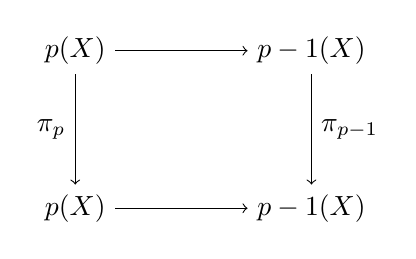
\begin{tikzpicture}[ auto]
      \node (A)  at (0,0) {$\DChains{p}(X)$};
      \node (B)  at (3,0) {$\DChains{p-1}(X)$};
      \node (C)  at (0,-2) {$\QDChains{p}(X)$};
      \node (D)  at (3,-2) {$\QDChains{p-1}(X)$};
      \draw[->] (A) to node {$\Boundary$} (B);
      \draw[->] (A) to node [swap] {$\pi_p$} (C);
      \draw[->] (B) to node {$\pi_{p-1}$} (D);
      \draw[->] (C) to node [swap] {$\Boundary$} (D);
    \end{tikzpicture}
  \end{center}
  where $\pi_p$ is the natural projection from $\DChains{p}(X)$ onto its quotient $\QDChains{p}(X)$.
  Moreover,
  the operator $\Boundary : \QDChains{p}(X) \to \QDChains{p-1}(X)$ again satisfies the boundary property $\Boundary \circ \Boundary = 0$.
\end{Article}

\begin{Article}{Cubic homology.}{}
  \label{Cubic-homology}
  Let $X$ be a diffeological space.
  As usual in homology theory \cite{McL75},
  when we have a chain complex,
  here $\QDChains{\star}(X)$ with $\star = 0,1, \ldots \infty$,
  and the boundary operator
  $$%
    \Boundary: \QDChains{\star}(X) \to \QDChains{\star-1}(X) \SpacedText{with} \Boundary \circ \Boundary = 0,
  $$%
  the space of \emph{$p$-cycles} is defined as the kernel in $\QDChains{p}(X)$ of the operator $\Boundary$,
  and the space of \emph{$p$-boundaries} as the image,
  in $\QDChains{p}(X)$,
  of the operator $\Boundary$ defined on $\QDChains{p+1}(X)$.
  These spaces will be denoted by
  $$%
    \left\{
    \begin{array}{rcll}
    \QDZ_p(X) & = &\ker[\Boundary \colon \QDChains{p}(X) \to
    \QDChains{p-1}(X)] & \mbox{with $p \geq 1$}, \\
    \QDB_p(X) & = & \Boundary (\QDChains{p+1}(X))\subset
    \QDZ_p(X) \subset \QDChains{p}(X) & \mbox{with $p \geq 0$.}
    \end{array}
    \right.
  $$%
  Then,
  the homology groups are defined as the quotients of the spaces of cycles by the spaces of boundaries
  $$%
    \QDH_p(X) = \QDZ_p(X)/\QDB_p(X).
  $$%
  Let us recall that for $p = 0$,
  $\Boundary \colon \QDChains{0}(X) \to \{0\}$,
  thus $\QDZ_0(X) = \QDChains{0}(X)$,
  and in this case $\QDH_0(X) =  \QDChains{0}(X)/\Boundary \QDChains{1}(X) = \DChains{0}(X)/\Boundary \QDChains{1}(X)$.
  We call this homology $\QDH_*(X)$,
  the \emph{cubic homology}%
  \footnote{In topology the cubic homology and the singular homology coincide \cite[Ex. 8.1]{HY61}
  For a natural singular homology in diffeology,
  these two homologies will coincide also.}
  of the space $X$.

  Once we have a homology,
  we get a cohomology,
  with values in $\RR$ for example,
  by a standard procedure \cite[\textsection\,6.63]{PIZ13}.

  A (real) \emph{cubic $p$-cochain of $X$} is a linear map
  $$%
    f \colon \DChains{p}(X) \to \RR
  $$%
  such that
  $$%
    f \colon \sum_{\sigma} n_\sigma \sigma \mapsto \sum_{\sigma} n_\sigma f(\sigma)
    \SpacedText{and}
    f \restriction \DCubes{p}(X) \in \Cinfty(\DCubes{p}(X),\RR),
  $$%
  The spaces of cubic $p$-cochains is denoted by $\DCochains{p}(X)$,
  that is,
  $$%
    \DCochains{p}(X) = \DHom(\DChains{p}(X),\RR) \simeq  \Cinfty(\DCubes{p}(X),\RR).
  $$%
  Now,
  the boundary $\Boundary$ defined from $\DChains{p+1}(X)$ to $\DChains{p}(X)$ induces,
  by duality,
  a {\em coboundary operator} $d$ such that
  $$%
    d : \DCochains{p}(X) \to  \DCochains{p+1}(X),
  $$%
  with
  $$%
    df(c) = f(\Boundary c)
  $$%
  for all $f \in \DCochains{p}(X)$,
  and all $c \in \DChains{p+1}(X)$.
  Then,
  by transfer of property,
  the coboundary $d$ satisfies
  $$%
    d \in \Hom(\DCochains{p}(X),\DCochains{p+1}(X))
    \SpacedText{and} d \circ d = 0.
  $$%
  The cohomology groups are defined by considering this operation applied to the reduced cubic chains,
  that is,
  by considering cochains defined on $\QDChains{p}(X)$,
  or which is equivalent,
  by considering the cubic cochains modulo \emph{reduced cochains},
  that is,
  the ones vanishing on reduced chains.
  That gives finally the \emph{cubic cohomology groups}\,:
  $$%
    \QDH^p(X,\RR) = \QDZ^p(X,\RR)/\QDB^p(X,\RR).
  $$%

  \uline{Note.} It is not clear if cubic (or singular) homology will play,
  in diffeology,
  the crucial role it plays in the theory of manifolds.
  But since it is a traditional tool,
  and since it is still a \emph{smooth invariant},
  it was worth extending it to the general case.
\end{Article} %% Cubic-homology

\begin{Article}{Integration on Chains.}
  Let $\sigma$ be a $p$-cube in $X$.
  Let $\alpha$ be a differential $p$-form on $X$,
  we \emph{integrate} $\alpha$ on $\sigma$ by
  $$%
    \int_\sigma \alpha = \int_{\Id_p} \alpha(\sigma) = \int_{\cub{p}} \sigma^*(\alpha)(\Id_p),
  $$%
  but $\sigma^*(\alpha)(\Id_p)$ is a smooth $p$-form on $\RR^p$,
  thus,
  there exists a smooth real function $f \in \Cinfty(\RR^p,\RR)$ such that
  $$%
     \sigma^*(\alpha)(\Id_p) = f\, \Vol_p = f(x_1,\dots,x_p) \, dx_1 \wedge \cdots \wedge dx_p.
  $$%
  and therefore,
  $$%
    \int_{\cub{p}} \sigma^*(\alpha)(\Id_p) = \int_{\cub{p}} f \Vol_p = \int_0^1 dx_1\cdots\int_0^1 dx_p \, f(x_1,\dots,x_p).
  $$%
  \uline{Definition.}{ \itshape The integration of a differential $p$-form $\alpha$ on $p$-chains defines a cochain,
  denoted here by $\overline\alpha$\,:
  $$%
    \overline\alpha(\sigma) = \int_\sigma \alpha
    \quad \Rightarrow \quad
    \overline\alpha\bigg(\sum_\sigma n_\sigma \sigma\bigg) =  \sum_\sigma n_\sigma \overline\alpha(\sigma) = \sum_\sigma n_\sigma \int_\sigma \alpha.
  $$%
  }
  It turns out that

  \uline{Theorem.}{ \itshape The differential $d$ on the cochain $\alpha$ coincides with the exterior derivative.
  This is the so-called \emph{Stokes' theorem} which is actually due to Sir William Thomson (1824--1907),
  known as Lord Kelvin:
  $$%
    \overline\alpha(\Boundary\sigma) = \overline{d\alpha}(\sigma),
    \SpacedText{that is,}
    \int_\sigma d\alpha = \int_{\Boundary \sigma} \alpha.
  $$%
  }
  That construction induces a morphism,
  called \emph{De Rham Morphism} in every degree $p$
  $$%
    \hdR^p \colon \HDR^p(X) \to \QDH^p(X,\RR).
  $$%
  One can check that
  $$%
    \HDR^0(X) = \QDH^0(X,\RR) = \Maps(\pi_0(X),\RR).
  $$%
  One can show also that
  $$%
    \hdR^1 \colon \HDR^1(X) \to \QDH^1(X,\RR)
  $$%
  is injective.
  However,
  $\hdR^1$ is not surjective as shows the example of the torus $\Torus_\alpha$\,:
  $$%
    \HDR^1(\Torus_\alpha) = \RR
    \SpacedText{and}
    \QDH^1(\Torus_\alpha,\RR) = \RR^2.
  $$%
  The cokernel of $\hdR^1$ is interpreted by the introduction of the \v{C}ech cohomology,
  see \cite{PIZ23}.
  It is the class of principal fiber bundles with group $(\RR,+)$ over $X$,
  equipped with a flat connection.
  This obstruction is the first characteristic class specific to diffeology,
  since every principal bundle with contractible fiber over a manifold is trivial.
  It is even a geometric interpretation of the cokernel of the morphism from $\HDR^1(X) $ to $\QDH^1(X,\RR)$ in general.
\end{Article}

\vfill
\centerline{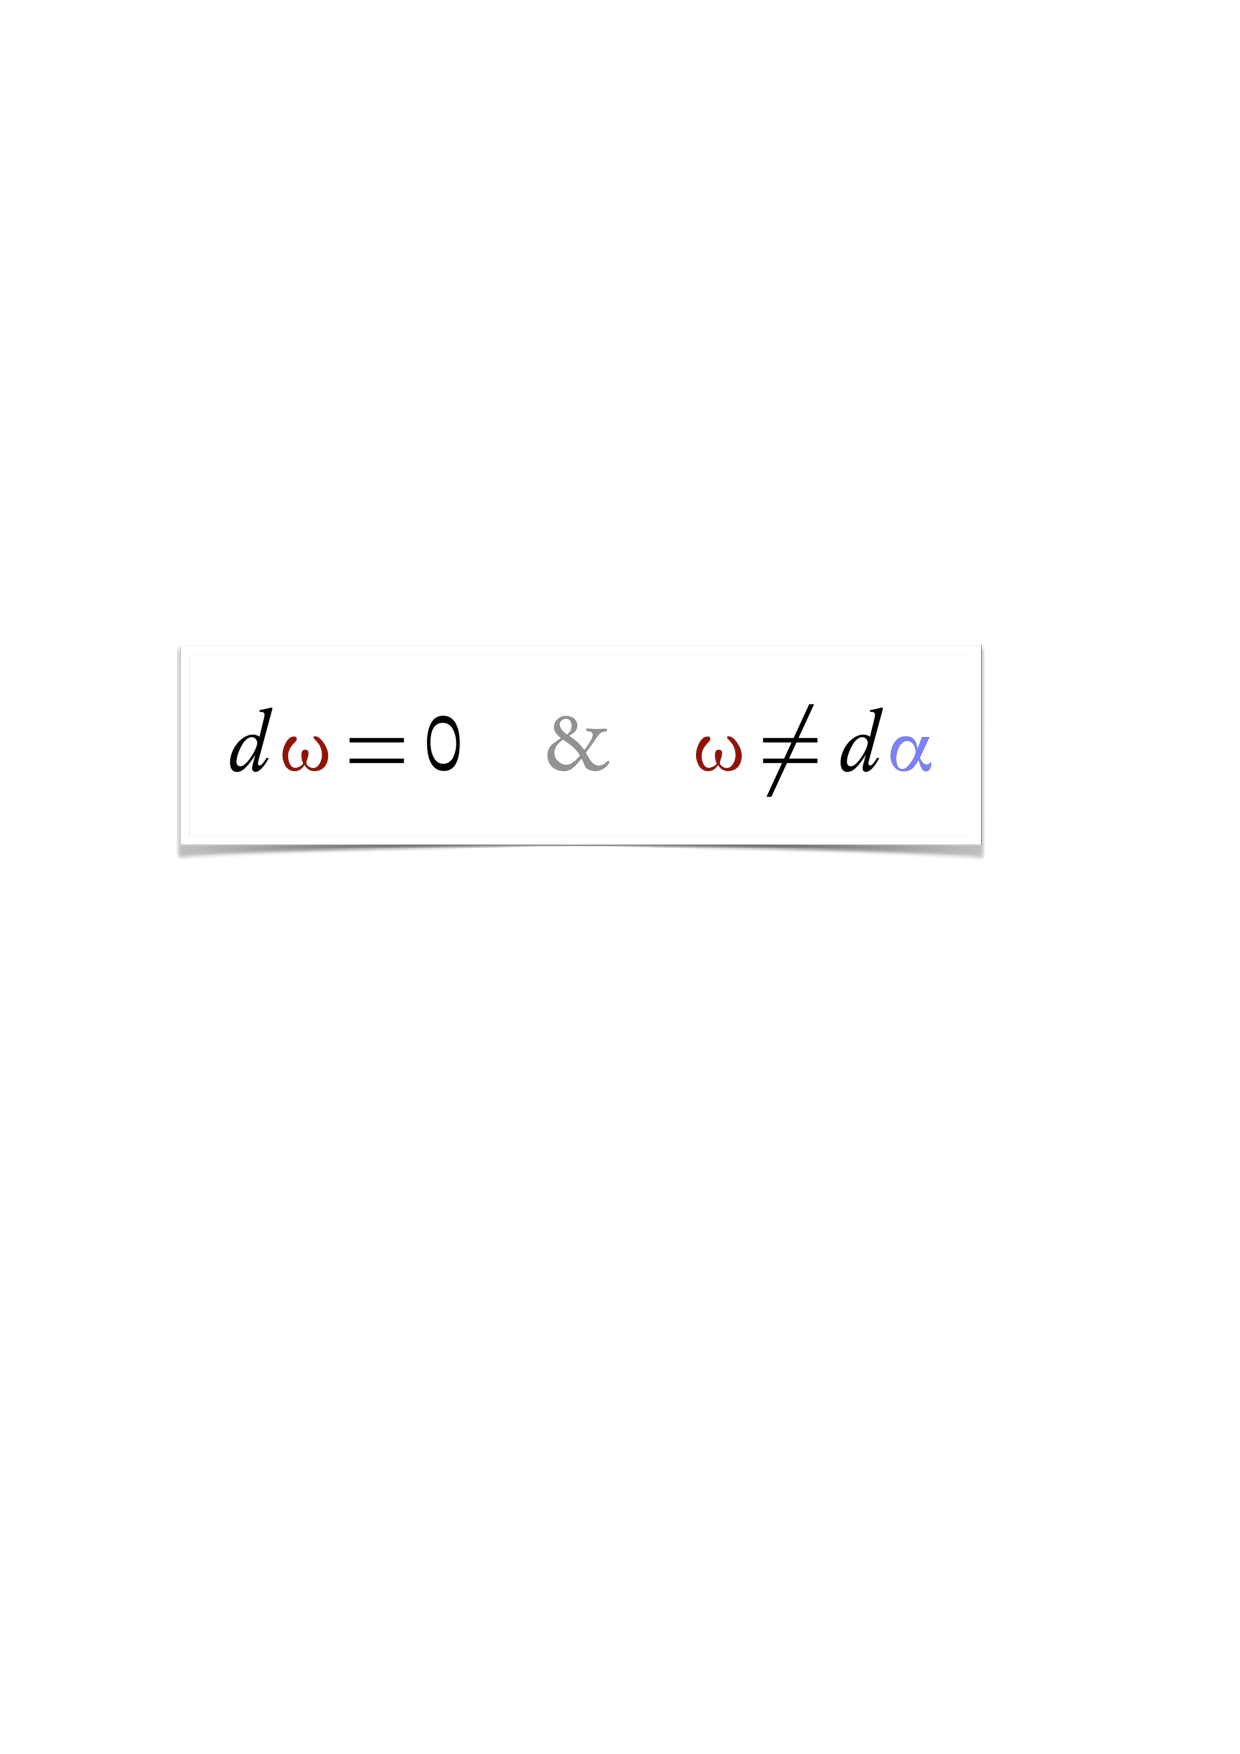
\includegraphics[width=1\textwidth]{Figures/domega.pdf}}
